% Start here


\chapter{Introduction}
\label{sec:intro}


The aim of this document is to report the results of the evaluation of the means of description to model the requirements of SUBSET-026 concerning the on-board unit and their associated tools.

This evaluation task is part on work package WP7, task 1  "Primary tool Chain analyses and recommendations". According to the results of WP2, especially the OpenETCS process and the requirements on language, the aim of this task is to determine the best candidates to  produce models of the on-board units, following the OpenETCS process

This process is described in details in D2.3 " Description of the openETCS process" and is summed up in the figure \ref{fig:main_process}. Requirements references quoted in the current document are defined in D2.6 "Requirements for openETCS".
 

 \begin{figure}
  \centering
  \fbox{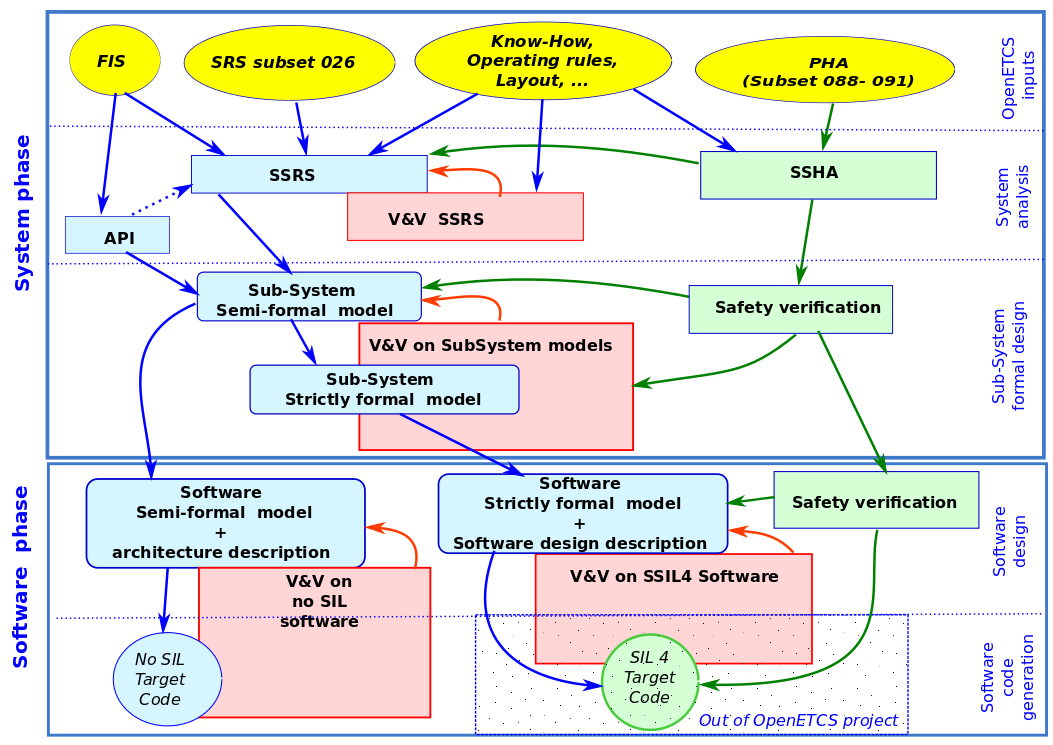
\includegraphics[scale=0.45]{WholeProcess.png}}
  \caption{Main OpenETCS process}
  \label{fig:main_process}
\end{figure}

Yellow elements are inputs, blue elements are part of the design process, red elements are verification and validation activities, green elements are safety activities. Each line (between dash or full blue lines) is a phase of the process, with a name on the right. 

The chapter \ref{sec:templates} of this document provides a template to describe the means and tools and a list of criteria according WP2 requirements on language, models and tools. The objectives of this description and criteria are to allow to determine the best means of description and associated tool for a given activities.

The chapter \ref{sec:concl} resumes the results of the evaluation at the end of the benchmark activities.

In Appendix, a chapter is dedicated to each models produced during the benchmark activities :
\begin{itemize}
\item  CORE
\item  GOPRR
\item  ERTMSFormalSpecs
\item  SysML with Papyrus
\item  SysML with Entreprise Architect
\item  SCADE
\item  EventB with Rodin
\item  Classical B with Atelier B
\item  Petri Nets
\item  System C
\item  GNATprove
\end{itemize}

For each approach and tool, the initial  author of the evaluation is the partner in charge of the modelling. Two assessors, for each approaches,  are in charge of the review of the evaluation and can correct it or add comments.

Tool platform are not covered by this document but in an other output of WP7 :  O7.1.9 "Evaluation of each tool platform against WP2 requirements, independent of target tools".
Besides, Task 7.1 is focussing on design activities : despite that some means can provide verification artefacts for example,  tools and means for validation, verification, test generation,... are in the scope of task 2 and will be analysed later.


%%%%%%%%%%%%%%%%%%%%%%%%%%%%%%%%%%%%%%%%%%%%%%%%%%%%%%%%%%%%%%%

\section{Reference Documents}
\label{sec:ref}

\begin{itemize}
\item CENELEC EN 50126-1 --- 01/2000 --- \emph{Railways applications –- The specification and
demonstration of Reliability, Availability, Maintainability and Safety (RAMS) –- Part 1:
Basic requirements and generic process}
\item CENELEC EN 50128 --- 10/2011 --- \emph{Railway applications -- Communication, signalling and
processing systems -- Software for railway control and protection systems}
\item CENELEC EN 50129 --- 05/2003 --- \emph{Railway applications –- Communication, signalling and
processing systems –- Safety related electronic systems for signalling}
\item D2.1 -- Report on existing methodologies 
\item D2.2 -- Report on CENELEC standards
\item D2.3 -- Definition of the overall process for the formal description of ETCS and the rail system it works in 
\item D2.4 -- Definition of the methods used to perform the formal description
\item D2.6 -- Requirements for OpenETCS
\end{itemize}


%%%%%%%%%%%%%%%%%%%%%%%%%%%%%%%%%%%%%%%%%%%%%%%%%%%%%%%%%%%%%%%

\section{Glossary}
\label{sec:glossary}

\begin{description}
\item[API] Application Programming Interface
\item[FME(C)A] Failure Mode Effect (and Criticity) Analysis
\item[FIS] Functional Interface Specification
\item[HW] Hardware
\item[I/O] Input/Output
\item[OBU] On-Board Unit
\item[PHA] Preliminary Hazard Analysis
\item[QA] Quality Analysis
\item[RBC] Radio Block Center
\item[RTM] RunTime Model
\item[SIL] Safety Integrity Level
\item[SRS] System Requirement Specification
\item[SSHA] Sub-System Hazard Analysis
\item[SSRS] Sub-System Requirement Specification
\item[SW] Software
\item[THR] Tolerable Hazard Rate
\item[V\&V] Verification \& Validation
\end{description}

%%%%%%%%%%%%%%%%%%%%%%%%%%%%%%%%%%%%%%%%%%%%%%%%%%%%%%%%%%%%%%%


